% Relatório de resultados — Oracle_N em diferentes níveis.
%
% Compile com:  tectonic -X compile relatorio.tex
%
% Cada seção vive em seu próprio arquivo sob secoes/, e o preâmbulo
% (pacotes e macros) em preambulo.tex. Para acrescentar uma seção, crie o
% arquivo e insira um \input abaixo, na posição em que ela deve aparecer.

\documentclass[11pt,a4paper]{article}

% Pacotes, geometria e macros compartilhados por todas as seções.
\usepackage[T1]{fontenc}
\usepackage[utf8]{inputenc}
\usepackage[brazil]{babel}
\usepackage[margin=2.5cm]{geometry}
\usepackage{booktabs}
\usepackage{graphicx}
\usepackage{amsmath,amssymb}
\usepackage{longtable}
\usepackage{array}
\usepackage{caption}
\usepackage{microtype}
\usepackage[hidelinks]{hyperref}

\newcommand{\On}[1]{\ensuremath{\text{Oracle}_{#1}}}
\newcommand{\dfe}{\ensuremath{\mathrm{DF}/e^{2}}}
\newcommand{\mvr}{MVR}


\title{\bfseries Análise do impacto de Oracles em diferentes níveis\\
na acurácia de Sistemas de Múltiplos Classificadores\\[0.4em]
\large Relatório de resultados --- respostas aos objetivos específicos}

\author{Subprojeto de Iniciação Científica}
\date{23 de agosto de 2026}

\begin{document}
\maketitle

\begin{abstract}
\noindent
Este relatório responde, um a um, aos oito objetivos específicos do subprojeto, a
partir de um experimento de $29$ bases $\times$ $10$ folds estratificados $\times$
$5$ modos de geração de pool ($1450$ folds, $0$ erros), com pools de $M=100$
classificadores. Três dos cinco modos separam o efeito do classificador-base do
efeito do método de geração --- um confounder de versões anteriores deste relatório
--- e um deles reativa a votação de medidas de complexidade do PGDCS completo,
antes desligada. As medidas \On{1} a \On{M} foram implementadas e verificadas; a
monotonicidade $\On{1}\ge\On{2}\ge\dots\ge\On{M}$ vale em $1450/1450$ folds, assim
como $\On{1}\ge$ votação majoritária. Os limites foram confrontados com a acurácia
individual, a votação majoritária, a média de probabilidades e \emph{doze} métodos
de seleção dinâmica de classificadores e de \emph{ensembles}.

Os quatro resultados centrais são: \textbf{(i)} o eixo que organiza os resultados é
o classificador-base, não o método de geração --- votar as medidas de complexidade
do PGDCS ou buscar com o algoritmo genético não muda \On{1}, $\mvr$ ou $\dfe$ de
forma estatisticamente sustentada ($p\ge0.13$ em todos os contrastes), e o padrão
inteiro (\On{1} alto, $\mvr$ baixo, folga grande) reaparece igual sem busca alguma,
some apenas quando o classificador-base muda para árvore; \textbf{(ii)} nenhum
nível intermediário de \On{N} serve como limite superior realista \emph{nos
problemas binários} --- o menor $N$ em que \On{N} cai abaixo da votação majoritária
fica em $N\approx M/2$ nos cinco modos (mediana $52$--$53$, Friedman $p=0.48$),
porque aí vale $\On{M/2+1}\le\mvr\le\On{M/2}$, verificado em $1100$ de $1100$ folds
binários; \textbf{(iii)} a folga $\On{1}-\mvr$ é previsível \emph{antes} de treinar
qualquer método de seleção, pelo índice de redundância de erros $\dfe$ (Spearman
$-0.89$, $n=145$), validado fora da amostra ($85{,}5\%$ de acerto
\emph{leave-one-dataset-out} contra $75{,}9\%$ da regra trivial); \textbf{(iv)}
mesmo tomando o melhor de dez métodos dinâmicos escolhido \emph{a posteriori} no
teste, a seleção dinâmica recupera entre $14{,}2\%$ e $24{,}3\%$ dessa folga,
conforme o modo --- o \On{1} é um limite inatingível na prática, não uma meta. O
relatório fecha com oito recomendações operacionais.
\end{abstract}


\tableofcontents
\bigskip

\section{Escopo e material}

O experimento cujos números este relatório reporta é o run canônico
\url{2026-08-24T09-38-20_5aceb11}, executado no commit \texttt{5aceb11}, de
árvore limpa (\texttt{git\_dirty: false}). Toda tabela, figura e teste aqui pode ser
reproduzido com

\begin{quote}\ttfamily\footnotesize
python scripts/run\_experiment.py --full\\
python scripts/analyze\_results.py results/experiments/<run>\\
python scripts/analyze\_review.py results/experiments/<run>
\end{quote}

\noindent
e conferido contra \texttt{analysis.txt}, \texttt{analysis.json} e
\texttt{review\_analysis.txt} gravados dentro do diretório do run. A análise textual
completa, com o encadeamento dos achados, está em
\path{docs/resultados-oracle-n.md}; este documento é o recorte que responde
diretamente às perguntas do subprojeto.

\paragraph{Procedência.} O run anterior (\texttt{2286fcc}) tinha
\texttt{git\_dirty: true} --- o código real divergia do commit registrado, e nada
publicado a partir dele era reproduzível (ADR 0019). O run canônico substitui-o de
árvore limpa. Antes de qualquer análise, os três modos comuns aos dois desenhos
(\texttt{ga}, \texttt{bagging}, \texttt{rf}) foram comparados coluna a coluna:
\textbf{$3480$ combinações base$\times$fold$\times$modo$\times$métrica de pool
comparadas, $0$ divergências, $\max|\Delta| = 0{,}000000000$}. O run sujo fica
\textbf{validado}: todo número já publicado sobrevive e ganha procedência
reprodutível.

\subsection{Protocolo}

\begin{table}[htbp]
\centering\small
\caption{Protocolo experimental.}
\begin{tabular}{ll}
\toprule
Item & Valor \\
\midrule
Bases & $29$ (das $31$ do catálogo; Ecoli e Glass excluídas pelo portão de viabilidade) \\
Validação & $10$-fold estratificado, \texttt{random\_state=42} \\
Partição interna & treino / validação-\emph{fitness} / DSEL, disjuntas \\
Tamanho do pool & $M=100$ em todos os modos \\
Modos de pool & PGDCS completo, PGDCS-F1/T1, bags aleatórios, Bagging, Random Forest \\
Fusores medidos & $14$ (MVR, combinação suave, $10$ dinâmicos, $2$ estáticos) \\
Métricas & acurácia, precisão e revocação macro, F1 macro, acurácia balanceada \\
Estatística & Friedman + Nemenyi (protocolo Dem\v{s}ar) e Wilcoxon pareado com Holm \\
Unidade pareada & a \emph{base} (folds promediados antes do teste) \\
Total & $1450$ folds, $0$ erros, $16$h$44$ de relógio \\
\bottomrule
\end{tabular}
\end{table}

Duas bases foram excluídas por um portão de viabilidade explícito: a classe mais
rara de Ecoli tem $2$ instâncias e a de Glass tem $9$, ambas abaixo dos $10$ folds,
o que impede a estratificação. A exclusão está registrada no manifesto do run com o
motivo, e não é um descarte silencioso.

\paragraph{Os cinco modos.} Cada um isola uma variável (ADR 0019):

\begin{description}
\item[PGDCS completo.] Perceptrons lineares, algoritmo genético, e a etapa em que o
método \emph{vota} quais medidas de complexidade convêm a cada base
(\texttt{get\_best\_types}) ativa --- a especificação original do método.
\item[PGDCS-F1/T1.] Idêntico, mas com as medidas fixas em F1 e T1 em vez de votadas.
É o modo já publicado em versões anteriores deste relatório; mantido para
comparabilidade e para o critério de aceitação do run acima.
\item[Bags aleatórios.] Mesmos bags estratificados de $50\%$, mesmo Perceptron,
mesma seed, \textbf{sem} busca genética --- a população de geração $0$ do próprio
GA. Isola o efeito da busca.
\item[Bagging.] Árvores de decisão sobre reamostragens \emph{bootstrap}.
\item[Random Forest.] Árvores com subamostragem adicional de atributos.
\end{description}

Os contrastes que os cinco modos destravam --- e cujos resultados aparecem nas
seções seguintes --- são: PGDCS completo \emph{vs} PGDCS-F1/T1 (efeito de votar as
medidas), PGDCS-F1/T1 \emph{vs} bags aleatórios (efeito da busca do GA), bags
aleatórios \emph{vs} Bagging (efeito do classificador-base).

\subsection{Definições usadas}

Para um pool com $M$ classificadores e uma amostra $x$,
\begin{equation}
\On{N}(x) = \mathbf{1}\!\left[\ \sum_{j=1}^{M} \mathbf{1}[\,h_j(x)=y(x)\,] \ \ge\ N \ \right],
\qquad N = 1,\dots,M ,
\end{equation}
de modo que \On{1} é o Oracle tradicional e vale
$\On{1}\ge\On{2}\ge\dots\ge\On{M}$.

Duas quantidades derivadas organizam o relatório:

\begin{description}
\item[Folga.] $\;\On{1}-\mvr$, a parcela do potencial anunciado pelo Oracle que a
votação majoritária não converte.

\item[Folga recuperada.] $\;\dfrac{\text{melhor método dinâmico}-\mvr}{\On{1}-\mvr}$,
a fração dessa folga que um método real alcança. O numerador usa o \emph{máximo por
fold} entre os dez métodos dinâmicos, escolhido no conjunto de teste: é um
\emph{oracle sobre métodos} e portanto uma cota superior generosa do que a seleção
dinâmica entrega.
\end{description}

Uma terceira quantidade mede diversidade de forma comparável entre pools de força
diferente. O Double Fault bruto (\texttt{DF}, a fração de pares que erram juntos)
penaliza pools fracos por construção, porque classificadores que erram mais erram
juntos mais. Normalizando pelo valor esperado sob erros independentes,
\begin{equation}
\dfe, \qquad e = 1 - \text{acurácia individual média},
\end{equation}
obtém-se um índice em que $1$ significa erros independentes e valores altos
significam redundância. O denominador acima assume taxa de erro igual entre
classificadores; a versão exata, $\frac{2}{M(M-1)}\sum_{i<j}e_ie_j$, é usada como
verificação de rigor na seção do objetivo 8.


%======================================================================
\section{Respostas aos objetivos específicos}

\subsection{Objetivo 1 --- o Oracle como limite superior em DCS/DES}

\textit{Estudar o conceito de Oracle em MCS, com ênfase em sua utilização como
medida de limite superior em técnicas de DCS e DES.}

O Oracle é o seletor ideal: dada uma amostra, ele escolhe um classificador correto
se existir algum no pool. Por isso é usado como cota superior de qualquer método de
seleção --- nenhum seletor real pode acertar uma amostra que \emph{nenhum} membro do
pool acerta. Souza e Cavalcanti (2017) documentam que essa cota é frouxa: técnicas
DCS selecionam classificadores competentes para no máximo cerca de $85\%$ das
instâncias, mesmo com Oracle de $100\%$ no treino.

O experimento reproduz e quantifica essa frouxidão nas $29$ bases. O \On{1} médio
fica entre $0.9951$ e $0.9976$ nos três modos --- ou seja, \emph{praticamente não
discrimina entre pools}. A informação está na distância até os métodos reais, não no
valor do Oracle. Esta é a motivação empírica direta da generalização proposta pelo
subprojeto e o fio condutor das seções seguintes.

\subsection{Objetivo 2 --- implementação do Oracle tradicional}

\textit{Implementar a medida tradicional de Oracle.}

Implementado em \texttt{pos/oracle/}, sobre uma matriz de acertos binária
$M \times n$ construída a partir das predições de cada classificador do pool. As
verificações que sustentam a corretude:

\begin{itemize}
\item $\On{1}\ \ge$ votação majoritária em \textbf{$1450/1450$ folds}. O Oracle
tradicional nunca subestimou um método real de combinação --- o que é uma
propriedade necessária, e sua violação indicaria erro na matriz de acertos.

\item Identidade de consistência, verificada com erro máximo $5.6\times10^{-16}$:
\begin{equation}
\frac{1}{M}\sum_{N=1}^{M}\On{N} \;\equiv\; \text{acurácia individual média do pool}.
\end{equation}
Ela decorre de $\sum_N P(\ge N \text{ corretos})/M = \mathbb{E}[\text{fração de
classificadores corretos}]$ e liga a curva à matriz de acertos por dois caminhos
independentes.
\end{itemize}

A identidade tem uma consequência metodológica que vale registrar: a
\textbf{``área sob a curva \On{N}'' não é uma métrica nova}. Ela é a acurácia média
dos classificadores-base sob outro nome, e não deve ser reportada como medida
independente.

\subsection{Objetivo 3 --- generalização para \On{N}}

\textit{Propor e implementar a generalização do Oracle em diferentes níveis.}

Implementada para todo $N=1,\dots,M$, com a curva completa gravada por fold. A
relação de monotonicidade $\On{1}\ge\On{2}\ge\dots\ge\On{M}$ --- que é a definição da
medida, não uma hipótese --- foi verificada em \textbf{$1450/1450$ folds, sem
exceção}.

\begin{table}[htbp]
\centering\small
\caption{Níveis de Oracle e métodos reais, média sobre $29$ bases $\times$ $10$ folds.}
\begin{tabular}{lrrrrrrr}
\toprule
Modo & \On{1} & \On{2} & \On{5} & \On{M} & \mvr & Comb.\ suave & Acc.\ indiv. \\
\midrule
PGDCS completo  & 0.9972 & 0.9953 & 0.9897 & 0.1139 & 0.7771 & 0.7752 & 0.7042 \\
PGDCS-F1/T1     & 0.9976 & 0.9963 & 0.9905 & 0.1179 & 0.7784 & 0.7738 & 0.7052 \\
Bags aleatórios & \textbf{0.9979} & 0.9957 & 0.9901 & 0.1158 & 0.7808 & 0.7768 & 0.7046 \\
Bagging         & 0.9951 & 0.9935 & 0.9884 & \textbf{0.3052} & 0.8467 & 0.8466 & 0.7931 \\
Random Forest   & 0.9970 & \textbf{0.9958} & \textbf{0.9920} & 0.1725 & \textbf{0.8549} & 0.8546 & 0.7806 \\
\bottomrule
\end{tabular}
\end{table}

A tabela já antecipa o problema central do objetivo 7: entre $N=1$ e $N=5$ a curva
cai apenas de $0.997$ para $0.990$, enquanto a votação majoritária está em
$0.78$--$0.85$. A faixa conservadora que o subprojeto procurava não está aqui.

\begin{figure}[htbp]
\centering
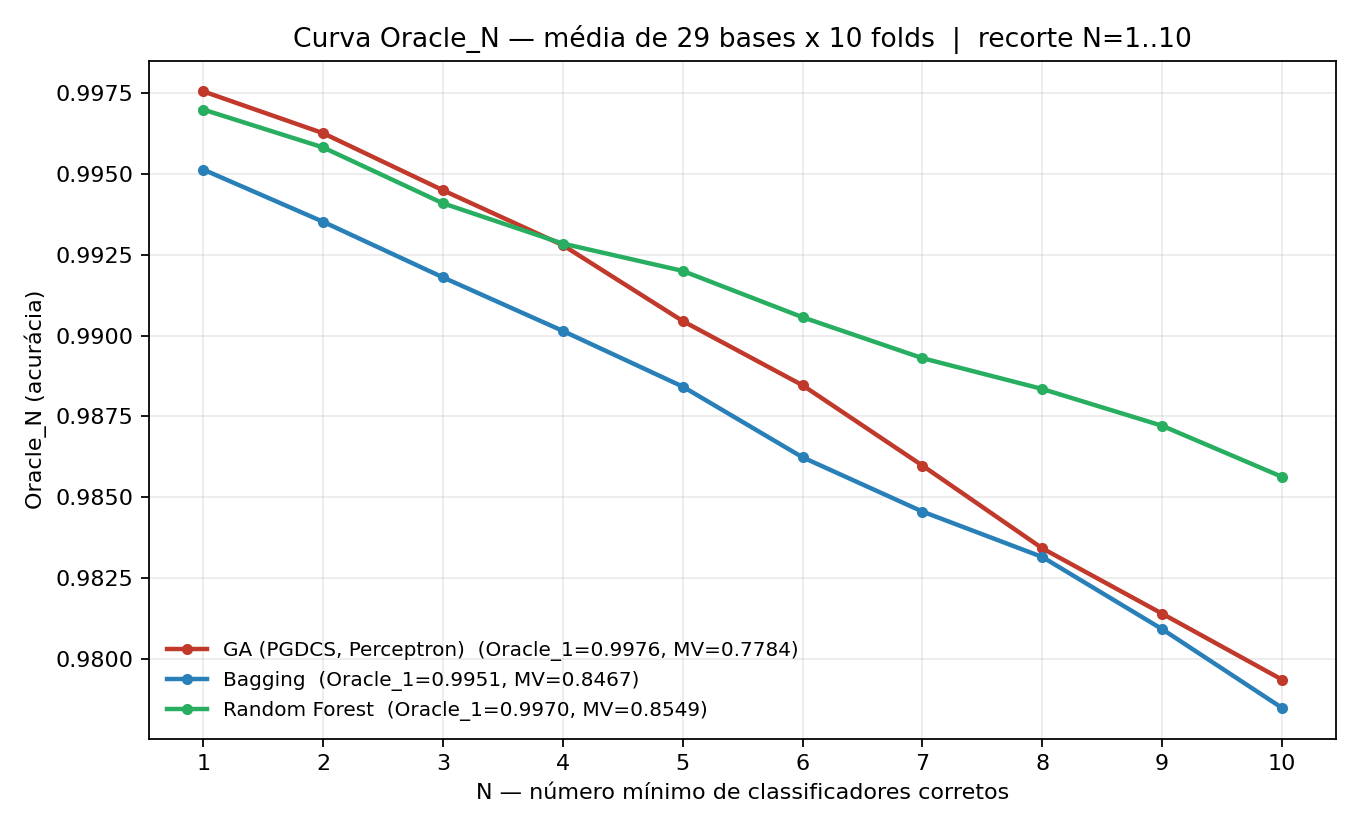
\includegraphics[width=0.86\textwidth]{figuras/fig2_oracle_curve_zoom.png}
\caption{Curva \On{N} no recorte $N=1..10$, com a votação majoritária de cada modo.
A distância vertical entre a curva e a linha tracejada correspondente é a folga.
Os três pools de Perceptron lideram em $N=1$, mas o Random Forest os ultrapassa a
partir de $N=3$: a vantagem do pool de menor acurácia individual existe só na ponta
mais otimista, e a Seção 5 mostra que ela não distingue entre os três métodos de
geração --- só entre classificadores-base.}
\end{figure}

\subsection{Objetivo 4 --- construção dos pools}

\textit{Construir pools com algoritmos simples e amplamente conhecidos, como Random
Forest e Perceptron, induzindo diversidade por variações de treinamento.}

Cinco modos, todos com $M=100$ (protocolo completo na Seção~1):

\begin{description}
\item[PGDCS completo.] Pool de Perceptrons lineares gerado por algoritmo genético
que otimiza medidas de complexidade dos \emph{bags}, com a etapa de votação das
medidas (\texttt{get\_best\_types}) ativa --- a especificação original do método.
\item[PGDCS-F1/T1.] Idêntico, com as medidas fixas em F1 e T1 em vez de votadas por
base. É a variante já publicada em versões anteriores deste relatório.
\item[Bags aleatórios.] Controle: mesmos bags, mesmo Perceptron, sem busca genética.
\item[Bagging.] Árvores de decisão sobre reamostragens \emph{bootstrap}.
\item[Random Forest.] Árvores com subamostragem adicional de atributos.
\end{description}

Os cinco atendem ao objetivo (algoritmos simples; diversidade por variação de
subconjuntos de dados, de atributos e da própria seleção dos \emph{bags}) e cobrem
uma faixa larga de força do classificador-base, o que se mostrou determinante nas
seções seguintes.

A medida de diversidade merece destaque porque o número bruto inverte a conclusão:

\begin{table}[htbp]
\centering
\caption{Diversidade: o Double Fault bruto contra o índice normalizado.}
\begin{tabular}{lrrrr}
\toprule
Modo & Acc.\ individual & DF bruto & $e^{2}$ esperado & \dfe \\
\midrule
PGDCS completo & 0.7042 & 0.1571 & 0.0875 & 2.12 \\
PGDCS-F1/T1    & 0.7052 & 0.1566 & 0.0869 & 2.13 \\
Bags aleatórios& 0.7046 & 0.1565 & 0.0873 & \textbf{2.10} \\
Random Forest  & 0.7806 & 0.1069 & 0.0481 & 2.92 \\
Bagging        & 0.7931 & 0.1094 & 0.0428 & 3.98 \\
\bottomrule
\end{tabular}
\end{table}

Pelo DF bruto os três pools de Perceptron seriam os \emph{menos} diversos (valores
mais altos, $\approx0.156$--$0.157$); pelo índice normalizado eles são os
\emph{mais} diversos (valores mais baixos, $2.10$--$2.13$; Friedman
$p=0.00026$, $k=5$). O DF absoluto sozinho leva ao diagnóstico errado, porque
classificadores mais fracos erram mais e portanto erram juntos mais.

\paragraph{O confounder geração $\times$ classificador-base, resolvido.} A versão
anterior deste relatório não podia separar ``o GA gera diversidade útil'' de ``o
Perceptron é mais fraco individualmente'' --- os dois efeitos andavam juntos.
Comparando os cinco modos par a par (Wilcoxon pareado por base, $N=29$):

\begin{table}[htbp]
\centering\small
\caption{Contrastes entre modos de geração --- nenhuma métrica difere entre PGDCS
completo, PGDCS-F1/T1 e bags aleatórios; todas diferem entre bags aleatórios e
Bagging.}
\begin{tabular}{lrrr}
\toprule
Contraste & \On{1} & $\mvr$ & $\dfe$ \\
\midrule
PGDCS completo \emph{vs} F1/T1 & $p=0.39$ & $p=0.88$ & $p=0.29$ \\
F1/T1 \emph{vs} bags aleatórios & $p=0.59$ & $p=0.15$ & $p=0.13$ \\
Bags aleatórios \emph{vs} Bagging & $p=0.12$ & $\mathbf{p=0.0038}$ & $\mathbf{p=0.0004}$ \\
\bottomrule
\end{tabular}
\end{table}

\textbf{Nenhuma das duas variáveis de geração dentro do Perceptron --- votar as
medidas de complexidade ou buscar com o GA --- produz uma diferença estatisticamente
sustentada em \On{1}, $\mvr$ ou $\dfe$.} A diferença aparece inteira no contraste
seguinte, bags aleatórios \emph{vs} Bagging: mesma ausência de busca dos dois lados,
único fator restante é o classificador-base, e é aí que $\mvr$ cai $0.066$ e $\dfe$
cai de $2.10$ para $3.98$. \textbf{O eixo que organiza os resultados deste
relatório é o classificador-base, não o método de geração.} A tese de que a busca
do GA por diversidade produz especialistas que a votação desperdiça não se sustenta
nestes dados: o mesmo padrão (\On{1} altíssimo, $\mvr$ baixo, folga grande) aparece
igual com ou sem busca, e some quando o classificador-base muda para árvore.

Isso também fecha, por medição, se o atalho \texttt{F1/T1} custa resultado: não
custa. Reativar a votação completa do PGDCS gastou $10{,}7$h de relógio
concentradas em duas bases (Magic e WDVG) para produzir um pool
estatisticamente indistinguível do que as medidas fixas já entregavam. Curiosamente,
a votação raramente escolhe F1/T1: o par aparece em apenas $4$ dos $290$ folds
($1{,}4\%$); os pares mais votados são combinações com F3, F4, LSC e N-medidas
(Seção~8, objetivo~7). O atalho não é uma boa adivinhação da votação --- é uma
substituição que, apesar de escolher medidas diferentes, chega ao mesmo resultado.

\subsection{Objetivo 5 --- avaliação experimental nas bases}

\textit{Avaliar o comportamento dos níveis de Oracle em bases públicas de
classificação.}

Foram usadas $29$ bases públicas (UCI, KEEL e as sintéticas clássicas da literatura
de MCS: P2, Banana, Lithuanian), com $178$ a $19\,020$ amostras, $2$ a $8$ classes e
razão de desbalanceamento de $1.0$ a $71.5$.

\paragraph{Ressalva explícita.} O objetivo 5 menciona preferência por \emph{bases de
imagens} públicas. O catálogo atual privilegia comparabilidade direta com a
literatura de referência (as $28$ bases de Monteiro et al., 2022, mais Magic) em vez
de bases de imagens. É um desvio consciente do enunciado, registrado aqui e nas
pendências do \texttt{ROADMAP}; incorporar bases de imagens é trabalho futuro
imediato, e não altera nenhum dos mecanismos identificados, que dependem da geometria
da fronteira e não do domínio.

\begin{figure}[htbp]
\centering
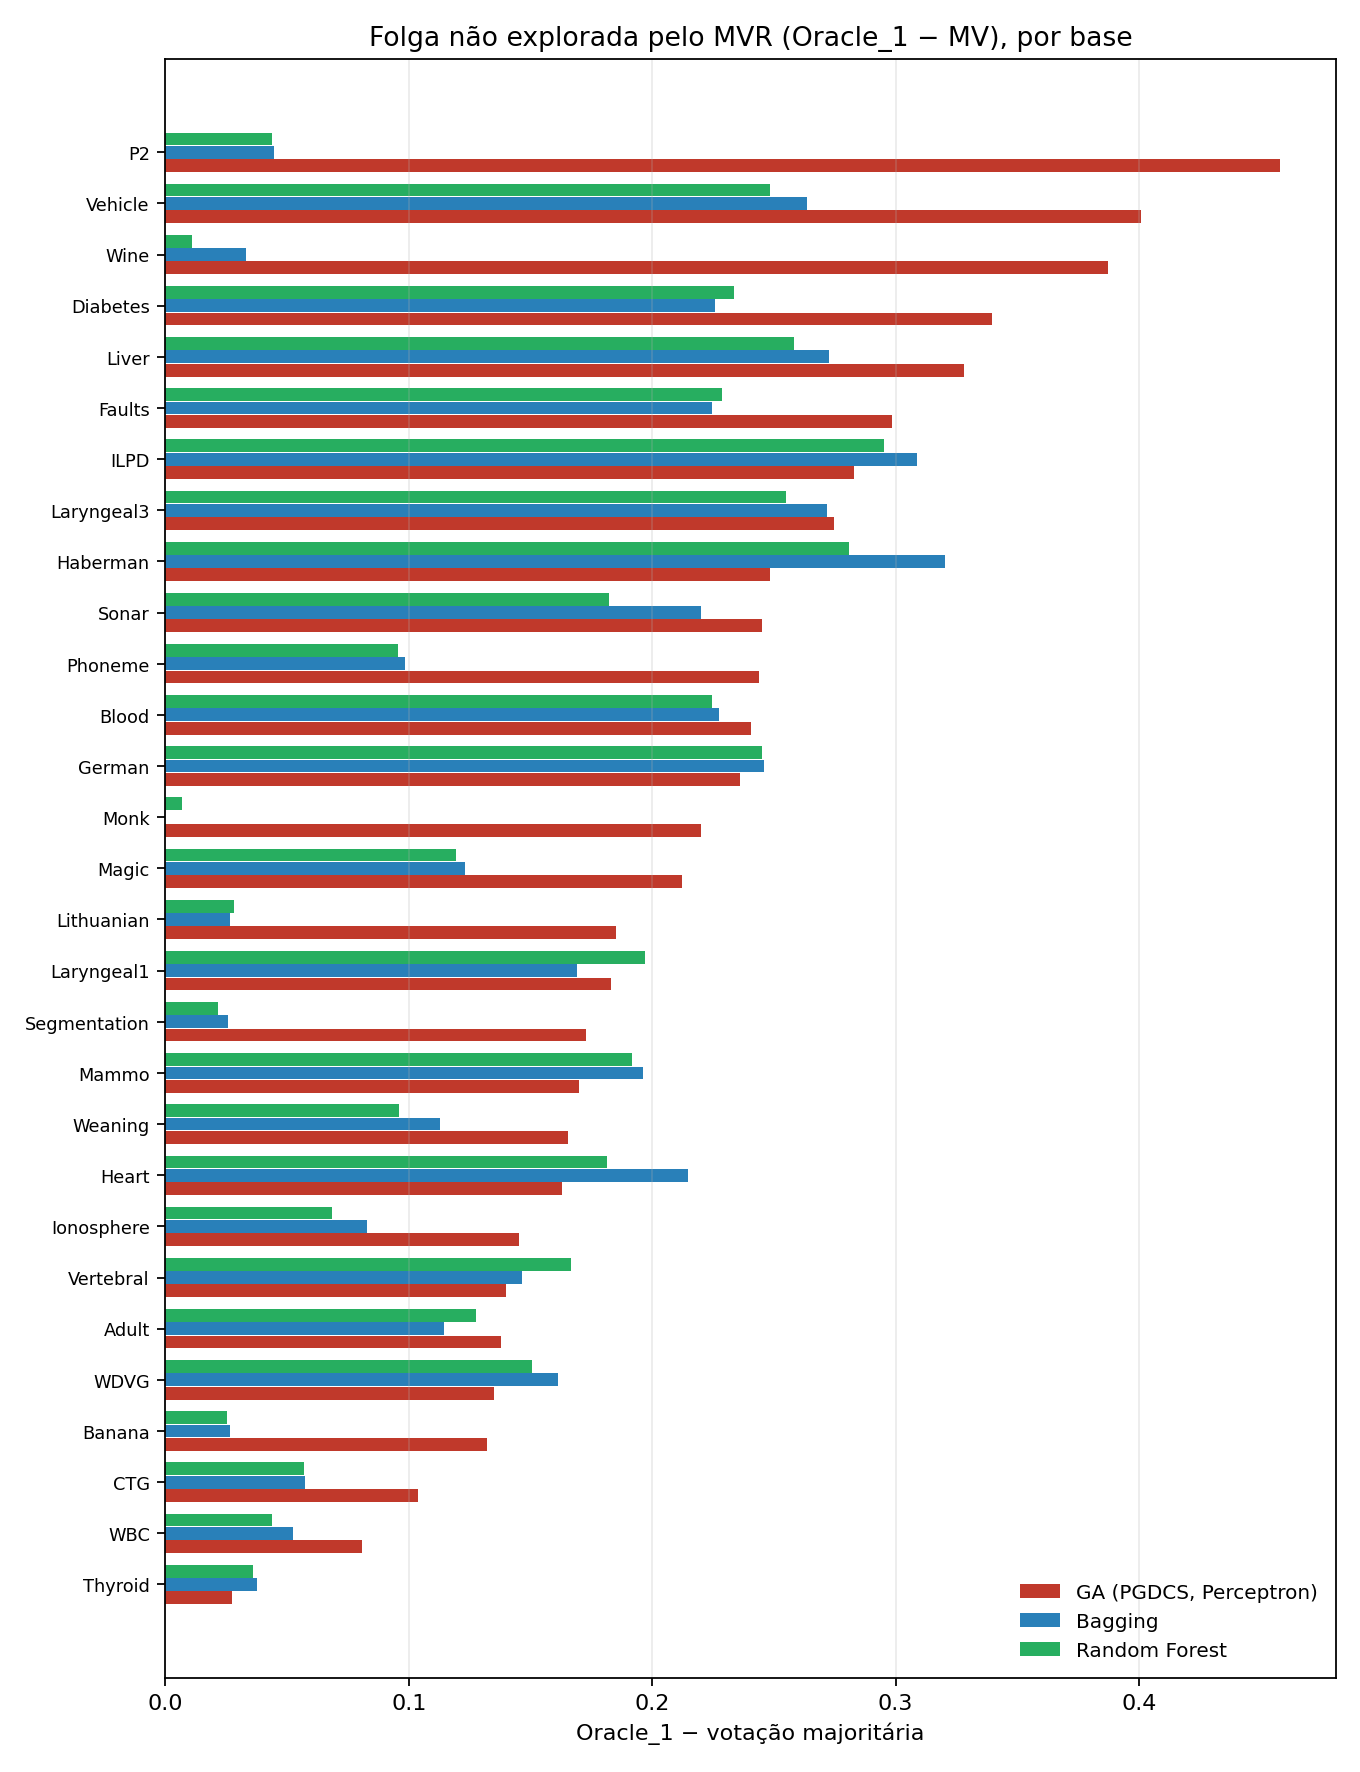
\includegraphics[width=0.92\textwidth]{figuras/fig4_gap_per_dataset.png}
\caption{Folga $\On{1}-\mvr$ por base. A dispersão entre bases ($0.017$ a $0.458$) é
muito maior que a dispersão entre modos ($0.142$ a $0.219$): o potencial não
explorado é sobretudo uma propriedade do problema, não da estratégia de geração.}
\end{figure}

\subsection{Objetivo 6 --- comparação com métodos reais}

\textit{Comparar a acurácia estimada pelos níveis de Oracle com classificadores
individuais e métodos reais de combinação (votação majoritária, média de
probabilidades) e, quando viável, DCS/DES.}

Foram medidos $14$ fusores nos $1450$ folds dos cinco modos, com DSEL disjunto e
$k=7$ vizinhos ($k=6$ nos pools de Perceptron, sem os dois métodos que exigem
\texttt{predict\_proba}). Esta seção detalha os três modos já publicados
(PGDCS-F1/T1, Bagging, Random Forest); o objetivo 4 (Seção~5) mostra que PGDCS
completo e bags aleatórios reproduzem o mesmo padrão do PGDCS-F1/T1 em todas as
métricas de pool, sem diferença estatística --- a tabela abaixo generaliza para os
três modos de Perceptron, não apenas o F1/T1.

\begin{table}[htbp]
\centering
\small
\caption{Acurácia média dos $14$ fusores contra o teto \On{1}. Traço $=$ método que
exige \texttt{predict\_proba}, indisponível no Perceptron linear.}
\begin{tabular}{lrrr}
\toprule
Fusor & PGDCS-F1/T1 & Bagging & Random Forest \\
\midrule
Votação majoritária (\mvr)      & 0.7784 & 0.8467 & 0.8549 \\
Combinação suave                & 0.7738 & 0.8466 & 0.8546 \\
\midrule
OLA                             & 0.7829 & 0.8028 & 0.7915 \\
LCA                             & 0.7271 & 0.7878 & 0.7863 \\
MCB                             & 0.7828 & 0.7943 & 0.7900 \\
Rank                            & 0.7760 & 0.8022 & 0.7908 \\
KNORA-E                         & 0.7897 & 0.8261 & 0.8274 \\
KNORA-U                         & \textbf{0.8056} & 0.8468 & \textbf{0.8564} \\
DES-P                           & 0.8021 & 0.8481 & 0.8566 \\
DES-KNN                         & 0.7995 & 0.8477 & 0.8492 \\
META-DES                        & ---    & \textbf{0.8482} & 0.8545 \\
KNOP                            & ---    & \textbf{0.8486} & 0.8556 \\
\midrule
Melhor individual (estático)    & 0.7630 & 0.7999 & 0.7958 \\
Seleção estática                & 0.7797 & 0.8475 & 0.8546 \\
\midrule
Melhor por fold (\emph{oracle} sobre métodos) & 0.8340 & 0.8688 & 0.8733 \\
Acurácia individual média       & 0.7052 & 0.7931 & 0.7806 \\
\On{1}                          & 0.9976 & 0.9951 & 0.9970 \\
\midrule
Folga $\On{1}-\mvr$             & 0.2192 & 0.1484 & 0.1421 \\
\textbf{Folga recuperada}       & \textbf{24.0\%} & \textbf{15.0\%} & \textbf{14.2\%} \\
\bottomrule
\end{tabular}
\end{table}

\begin{figure}[htbp]
\centering
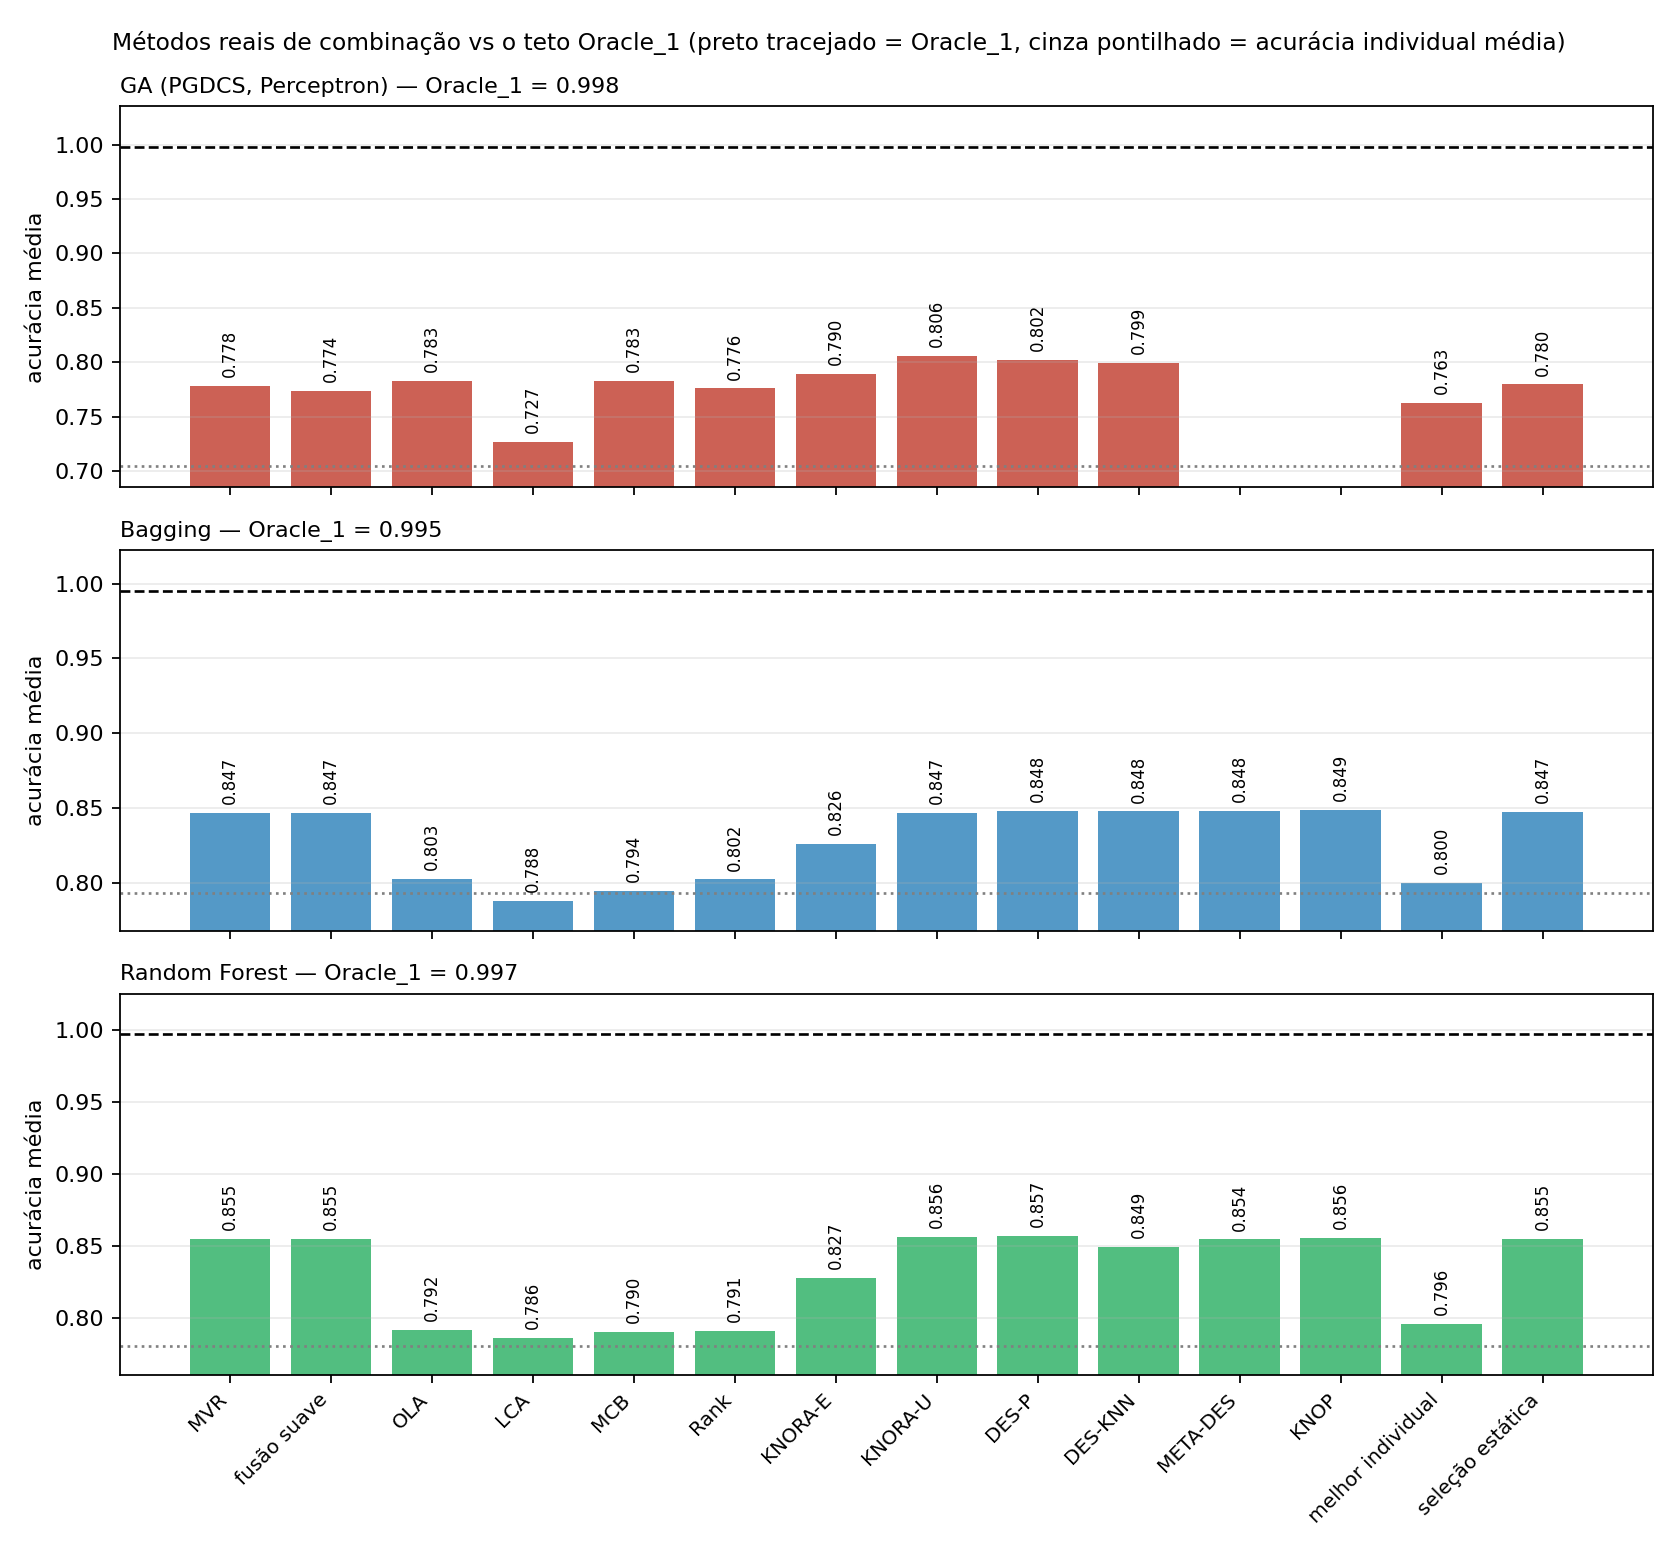
\includegraphics[width=0.95\textwidth]{figuras/fig7_fuser_accuracy.png}
\caption{Os $14$ fusores contra o teto \On{1} (tracejado preto) e a acurácia
individual média (pontilhado cinza), um painel por modo. A distância da barra mais
alta até a linha tracejada é a parte do potencial do pool que nenhum método
alcançou. Barra ausente $=$ método inaplicável ao pool.}
\end{figure}

\paragraph{(a) O melhor pool produz a pior votação.}
O PGDCS-F1/T1 tem o \emph{maior} \On{1} entre os pools de árvore e Perceptron
publicados aqui ($0.9976$) e a \emph{menor} votação majoritária de todas
($0.7784$). A folga resultante, $0.2192$, é $48\%$ maior que a do Random Forest
(Friedman $p=0.0022$, $k=5$; PGDCS-F1/T1 \emph{vs} RF acima da diferença crítica,
Wilcoxon $p=0.0003$). Em P2 o pool contém um classificador correto para
\emph{toda} amostra de teste ($\On{1}=1.0000$), os erros são praticamente
independentes ($\dfe=1.02$) e a votação majoritária entrega $0.5420$. Não é falta de
informação no pool --- é o fusor que não a extrai.

\paragraph{(b) A combinação suave não supera a votação majoritária em nenhum modo.}
Nos pools de árvores as duas regras empatam ($\Delta$ da ordem de $10^{-4}$; dão o
mesmo resultado em $278$ e $275$ dos $290$ folds). No pool de Perceptrons a
combinação suave é pior em média ($-0.0046$), mas a diferença \textbf{não é
estatisticamente significativa} ($p=0.51$). A conclusão que se sustenta é a negativa:
para pools de classificadores lineares a média de margens normalizadas não é o
método real a bater --- o \mvr{} é.

\paragraph{(c) O eixo que organiza a seleção dinâmica é a poda.}
O resultado mais robusto do experimento não é sobre a folga, é sobre o custo de
descartar membros do pool. Testando cada fusor contra o \mvr{} por base ($N=29$),
com correção de Holm para a família de $13$ testes:

\begin{table}[htbp]
\centering
\small
\caption{Fusores contra o \mvr{} no pool Random Forest (Wilcoxon pareado, Holm).}
\begin{tabular}{lrrcr}
\toprule
Fusor & Média & $\Delta$ \emph{vs} \mvr & Vitórias/derrotas & $p$ (Holm) \\
\midrule
LCA                & 0.7863 & $-0.0686$ & 0/29 & $<0.001$ \\
MCB                & 0.7900 & $-0.0649$ & 0/29 & $<0.001$ \\
Rank               & 0.7908 & $-0.0641$ & 0/29 & $<0.001$ \\
OLA                & 0.7915 & $-0.0634$ & 0/29 & $<0.001$ \\
Melhor individual  & 0.7958 & $-0.0592$ & 1/28 & $<0.001$ \\
KNORA-E            & 0.8274 & $-0.0275$ & 3/24 & $0.0004$ \\
DES-KNN            & 0.8492 & $-0.0057$ & 10/18 & 0.097 \\
KNORA-U            & 0.8564 & $+0.0015$ & 19/6 & 0.31 \\
DES-P              & 0.8566 & $+0.0017$ & 13/9 & 0.84 \\
KNOP               & 0.8556 & $+0.0006$ & 13/12 & 1.00 \\
META-DES           & 0.8545 & $-0.0005$ & 13/15 & 1.00 \\
Seleção estática   & 0.8546 & $-0.0003$ & 14/12 & 1.00 \\
Combinação suave   & 0.8546 & $-0.0003$ & 1/2 & 1.00 \\
\bottomrule
\end{tabular}
\end{table}

Em Bagging o padrão é idêntico: OLA, LCA, MCB e Rank perdem em $27$--$28$ das $28$
bases, com $\Delta$ entre $-0.044$ e $-0.059$ e $p_{\text{Holm}}\le 0.0001$. A escala
é clara:

\begin{itemize}
\item podar até \emph{um} classificador (OLA, LCA, MCB, Rank, melhor individual)
$\rightarrow$ perda de $0.044$ a $0.069$ nos pools de árvores, sempre significativa;
\item podar parcialmente (KNORA-E) $\rightarrow$ perda intermediária, ainda
significativa;
\item não podar, apenas reponderar (KNORA-U, DES-P, META-DES, KNOP, seleção
estática) $\rightarrow$ empate técnico com o \mvr.
\end{itemize}

Os dois métodos estáticos confirmam o eixo pelos extremos: a seleção estática, que
mantém o pool inteiro, empata com o \mvr{} nos três modos; o melhor individual, que
é poda máxima sem nenhuma localidade, está entre os piores em todos.

\paragraph{(d) Onde a seleção dinâmica de fato paga.}
No pool de Perceptrons a ordem se inverte parcialmente: \textbf{KNORA-U é o único
fusor que supera o \mvr{} de forma estatisticamente sustentada em algum modo}
($+0.0272$, $p_{\text{Holm}}=0.0045$, vencendo em $147$ dos $290$ folds contra $49$
derrotas e $94$ empates). Nos pools de árvores o mesmo método fica em $+0.0001$ e
$+0.0015$, sem significância.

A vantagem se concentra nas bases de fronteira não-linear em baixa dimensão: em P2,
Lithuanian e Banana a recuperação média do PGDCS-F1/T1 é $0.766$, contra $0.157$ do Bagging e
$0.155$ do Random Forest nas mesmas bases. O mecanismo é geométrico: um Perceptron
não separa a espiral do P2, mas separa qualquer vizinhança dela, e escolher o
Perceptron certo por região é exatamente o que falta. Uma árvore já resolve a
fronteira sozinha, então o voto majoritário já está perto do que o pool consegue e
não sobra folga \emph{local} a extrair.

\paragraph{(e) O viés de estimação foi medido, não apenas discutido.}
Numa versão anterior do protocolo o DSEL da seleção dinâmica era a mesma partição
que o PGDCS-F1/T1 usa na função de \emph{fitness}, o que favorecia o PGDCS-F1/T1 por construção. O
protocolo atual separa as duas partições. Isolar o viés exige separar dois efeitos
simultâneos --- o viés removido (só afeta o PGDCS-F1/T1) e o DSEL pela metade (afeta os três
modos) --- e Bagging e RF servem de grupo de controle, porque mantêm os pools
\emph{bit-idênticos} entre os dois desenhos (verificado: $\max|\Delta| = 0.000000$
em toda coluna de pool e curva Oracle idêntica em $290/290$ folds de cada modo).

Pela diferença-em-diferenças, restrita aos cinco métodos comuns aos dois desenhos: o
controle perdeu $-0.0057$ de folga recuperada, o PGDCS-F1/T1 perdeu $-0.0003$, logo o viés é
$+0.0055$ --- cerca de $3\%$ relativos, e nenhum dos deltas é significativo. O
desenho anterior \textbf{não} estava inflando materialmente a vantagem do PGDCS-F1/T1; a
correção está feita e é a que vale, mas não muda conclusão alguma.

\subsection{Objetivo 7 --- níveis intermediários são um limite mais realista?}

\textit{Analisar se níveis intermediários de Oracle podem representar estimativas de
limite superior mais conservadoras e mais próximas do desempenho de métodos reais.}

\textbf{A resposta é não}, e o experimento identifica a razão estrutural.

Defina $N^{*}$ como o menor $N$ tal que $\On{N} <$ votação majoritária --- o nível em
que o Oracle deixa de ser otimista.

\begin{table}[htbp]
\centering
\caption{$N^{*}$ por modo, com $M=100$.}
\begin{tabular}{lrrrr}
\toprule
Modo & Mediana & IQR & Média & Folds com $N^{*}>50$ \\
\midrule
GA            & 52 & $[51, 55]$ & 51.9 & 79.3\% \\
Bagging       & 53 & $[51, 56]$ & 54.4 & 81.4\% \\
Random Forest & 53 & $[51, 56]$ & 53.0 & 79.3\% \\
\bottomrule
\end{tabular}
\end{table}

Friedman $p=0.40$: \textbf{os três modos têm o mesmo $N^{*}$, e ele fica em
$N\approx M/2$}. Não é coincidência empírica. O mecanismo não é a identidade
$\On{M/2+1}\equiv\mvr$ --- essa afirmação, feita em versões anteriores, é falsa ---
mas um \emph{sanduíche}:
\begin{equation}
\On{M/2+1} \;\le\; \mvr \;\le\; \On{M/2}.
\end{equation}

A votação acerta sempre que mais da metade do pool acerta, logo $\mvr\ge\On{51}$;
e ela só pode ganhar, além disso, os empates $50$--$50$, logo nunca passa de
$\On{50}$. O sanduíche foi verificado em \textbf{660 de 660} folds binários, mas a
igualdade $\mvr=\On{51}$ vale em apenas $508$ deles ($77\%$): nos demais $23\%$ os
empates são desfeitos a favor, com excesso médio de $+0.0035$.

A distinção não é um detalhe --- é ela que dá o valor de $N^{*}$. Como $N^{*}$ é o
primeiro nível \emph{estritamente} abaixo do \mvr{}, e $\On{51}=\mvr$ não satisfaz
``$<$'', os empates empurram $N^{*}$ de $51$ para $52$ ou mais, que é exatamente
onde as medianas caem.

\paragraph{O limite é do caso binário.} $22$ das $29$ bases são binárias. Nas $7$
multiclasse a votação é por pluralidade e um classificador correto não precisa de
$51$ votos para vencer, então o sanduíche não vale --- e $N^{*}$ desce de forma
significativa:

\begin{table}[htbp]
\centering
\caption{$N^{*}$ mediano por cardinalidade de classes.}
\begin{tabular}{lrrrr}
\toprule
grupo & bases & GA & Bagging & RF \\
\midrule
binárias    & 22 & 53.4 & 53.7 & 53.5 \\
multiclasse &  7 & 44.4 & 48.1 & 47.3 \\
\bottomrule
\end{tabular}
\end{table}

\noindent
Mediana $53.7$ contra $47.6$, Mann-Whitney $p=2.7\times10^{-6}$. Dentro de cada
grupo os modos continuam empatados ($p=0.71$ e $p=0.37$).

Disso decorre a resposta ao objetivo, \textbf{restrita aos problemas binários}:

\begin{itemize}
\item Para $N \ll M/2$ a curva está \textbf{saturada}: os três modos ficam entre
$0.988$ e $0.998$ em $N=1..5$, e $\On{5}\ge\mvr$ em $100\%$ dos $870$ folds. As
diferenças entre modos são estatisticamente reais ($p<0.001$) mas de magnitude
$0.002$--$0.004$. Mais conservador que \On{1}, sim; perto de um método real, não.

\item Para $N\approx M/2$ a curva \textbf{já é} a votação majoritária, sob outro
nome. Não acrescenta informação.

\item \textbf{Não existe faixa intermediária útil} entre as duas.
\end{itemize}

\begin{figure}[htbp]
\centering
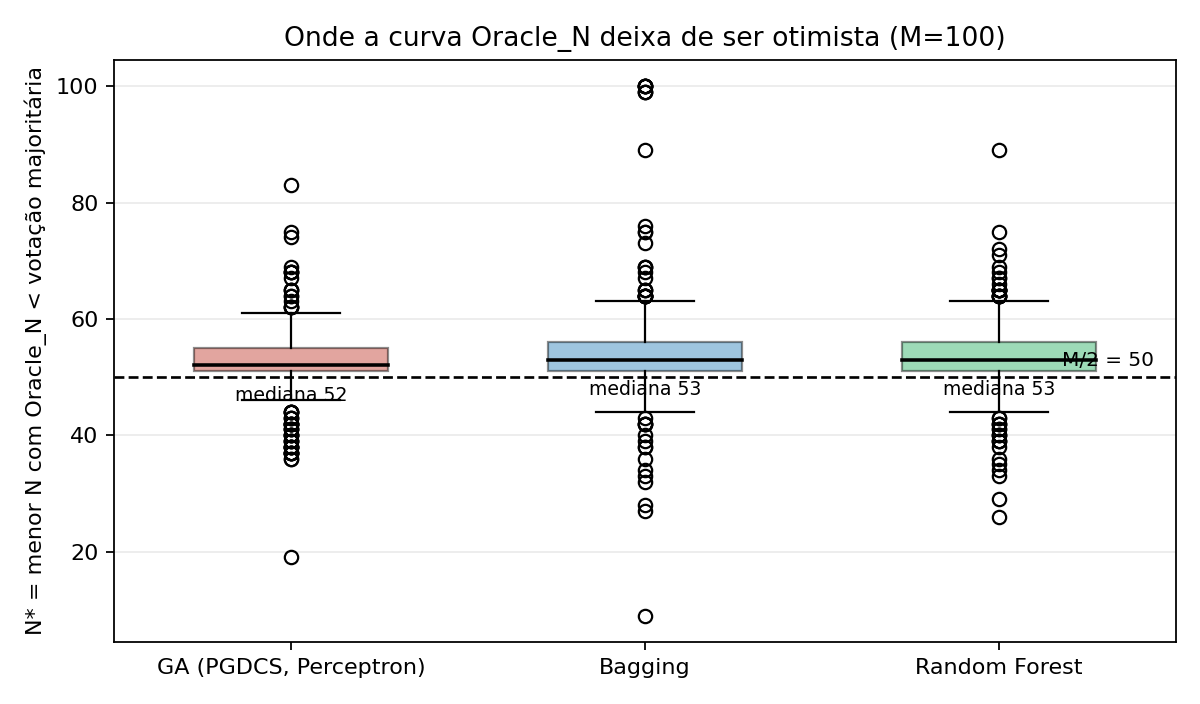
\includegraphics[width=0.72\textwidth]{figuras/fig3_nstar.png}
\caption{Distribuição de $N^{*}$. A concentração em torno de $M/2$ nos três modos é o
que impede qualquer nível intermediário de servir como limite realista.}
\end{figure}

\paragraph{O que substitui a ideia original.} O objetivo 7 buscava uma estimativa
conservadora e alcançável. Ela existe, mas não é ``\On{N} para algum $N$''; é a folga
$\On{1}-\mvr$ ponderada pela fração dela que métodos reais recuperam. Medido: mesmo
tomando o melhor de dez métodos dinâmicos escolhido \emph{a posteriori} no teste, a
recuperação fica em $24.0\%$ (GA), $15.0\%$ (Bagging) e $14.2\%$ (RF), com medianas
bem menores ($0.167$, $0.108$, $0.091$) e recuperação \emph{exatamente zero} no
primeiro quartil de Bagging e RF.

\textbf{Correção.} Versões anteriores apresentavam
\begin{equation}
\mvr + 0.15\,\bigl(\On{1}-\mvr\bigr)
\end{equation}
como ``limite superior operacional''. Não é um limite: $0.15$ é a recuperação
\emph{média} dos pools de árvore, e uma média é ultrapassada por metade da massa.
Medido nos folds de árvore, $37.7\%$ deles recuperam mais que $0.15$. A expressão é
uma \textbf{estimativa}, $\widehat{\mathrm{Acc}}_{DS}$, e deve ser lida como tal.

Quem quiser de fato uma cota precisa de um quantil alto da distribuição de
$R=\text{recuperação}$, não da sua média:
\begin{equation}
\widehat{\mathrm{Acc}}_{DS} = \mvr + \overline{R}\,\bigl(\On{1}-\mvr\bigr),
\qquad
\mathrm{cota}_{95} = \mvr + Q_{0.95}(R)\,\bigl(\On{1}-\mvr\bigr),
\end{equation}
com $Q_{0.95}(R)=0.50$ nos pools de árvore --- mais de três vezes a média. E os dois
números descrevem a mesma distribuição em que $31\%$ dos folds recuperam
\emph{nada} ($R\le 0$). Ambos permanecem otimistas, porque $R$ é medido escolhendo o
melhor método no próprio teste.

\paragraph{Robustez à métrica.} A metodologia do subprojeto pede precisão, revocação,
F1 e acurácia balanceada além da acurácia --- a preocupação legítima sendo que a
acurácia bruta esconda a classe minoritária, num catálogo que chega a IMB $71.5$. As
quatro métricas foram gravadas para \emph{todo} fusor. Em acurácia balanceada tudo
cai, mas de forma quase uniforme, e a folga \emph{cresce}:

\begin{table}[htbp]
\centering
\caption{Acurácia \emph{versus} acurácia balanceada.}
\begin{tabular}{lrrrrrr}
\toprule
Modo & \On{1} & \On{1} balanc. & \mvr & \mvr balanc. & Folga & Folga balanc. \\
\midrule
GA            & 0.9976 & 0.9967 & 0.7784 & 0.7368 & 0.2192 & 0.2599 \\
Bagging       & 0.9951 & 0.9923 & 0.8467 & 0.8163 & 0.1484 & 0.1760 \\
Random Forest & 0.9970 & 0.9949 & 0.8549 & 0.8214 & 0.1421 & 0.1735 \\
\bottomrule
\end{tabular}
\end{table}

O \On{1} é quase insensível ao desbalanceamento --- basta \emph{um} classificador do
pool acertar a instância minoritária --- enquanto o \mvr{} precisa que $51$ acertem,
e é aí que a minoria se perde. Nos \emph{ranks} de fusor a única mudança sistemática
é o DCS puro melhorar $0.3$--$0.4$ posições (OLA vai de \emph{rank} $6.38$ para
$6.00$ no RF), o que faz sentido --- escolher o competente na vizinhança ajuda numa
região minoritária. Mas em nenhum modo isso muda o topo: KNORA-U, META-DES, \mvr{} e
combinação suave continuam empatados na frente, e OLA e LCA continuam no fundo.
\textbf{Nenhuma conclusão deste relatório depende da escolha da métrica.}

\subsection{Objetivo 8 --- recomendações e redução de custo}

\textit{Gerar recomendações sobre o uso de Oracles em diferentes níveis como
ferramenta de análise prévia do potencial de desempenho de ensembles, considerando a
redução de custo computacional.}

A base quantitativa da recomendação é que o índice de redundância prevê a folga
\emph{antes} de treinar qualquer método de seleção:
\begin{equation}
\text{Spearman}\bigl(\dfe,\ \On{1}-\mvr\bigr) = -0.860,
\quad p = 8\times10^{-27},\quad n = 87 .
\end{equation}
Por modo: GA $-0.933$, Bagging $-0.909$, RF $-0.785$. O índice custa
$O(M^{2}n)$ sobre a matriz de acertos que já se tem.

\begin{figure}[htbp]
\centering
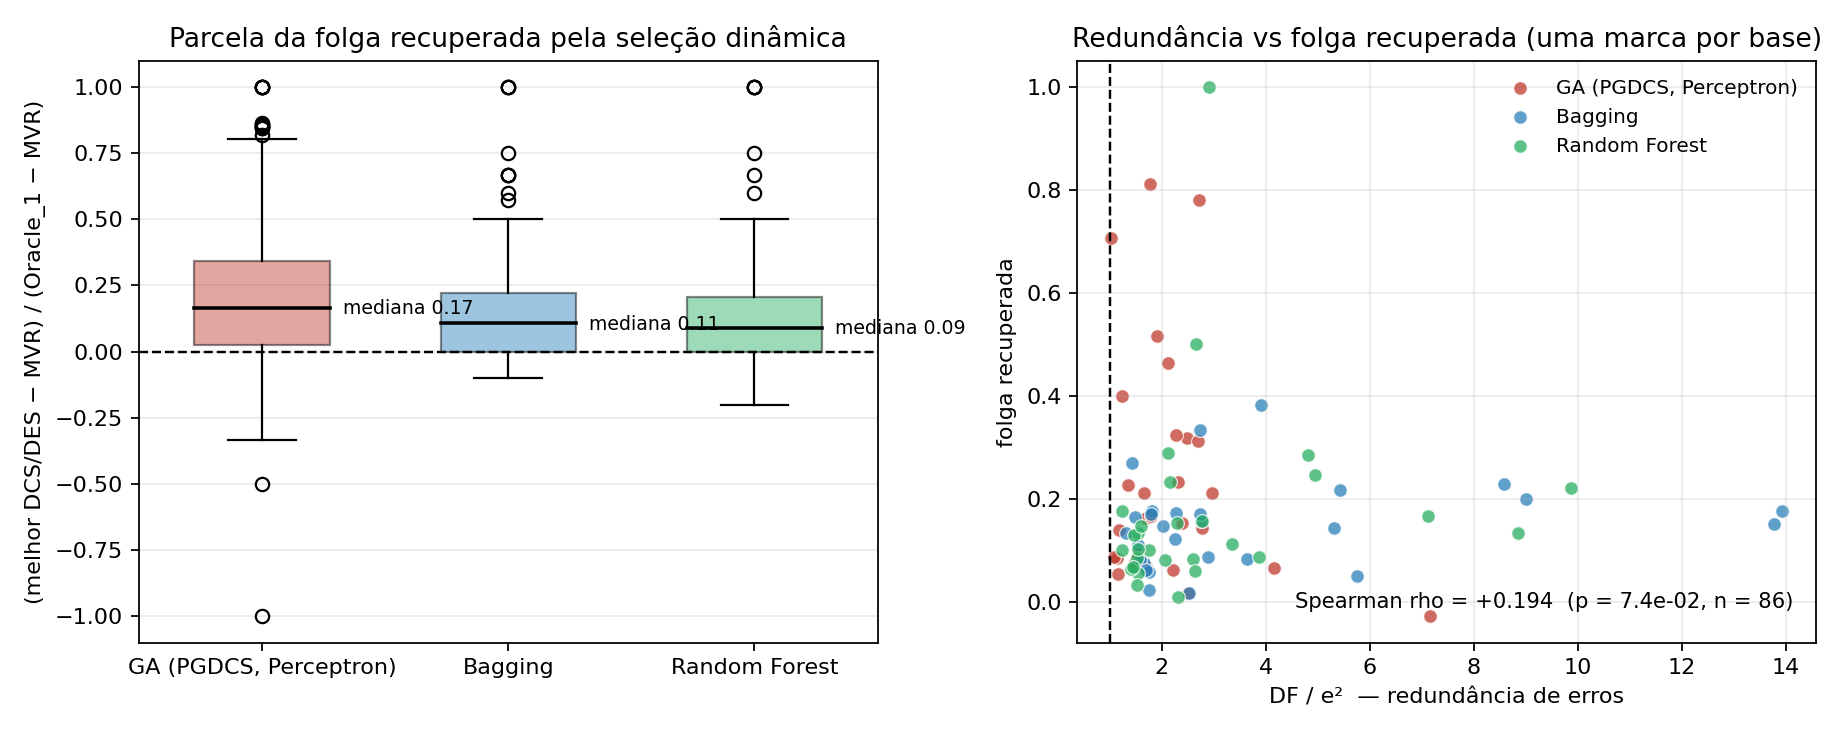
\includegraphics[width=0.95\textwidth]{figuras/fig8_recovered_gap.png}
\caption{À esquerda, a distribuição da folga recuperada por modo. À direita, a mesma
quantidade contra $\dfe$: a correlação que prevê o \emph{tamanho} da folga
não prevê a \emph{fração alcançável}.}
\end{figure}

As sete recomendações que o experimento sustenta:

\begin{enumerate}
\item \textbf{Use $\On{1}-\mvr$ como medida de potencial, não \On{1} como meta.}
O \On{1} fica entre $0.995$ e $0.998$ nos três modos e $29$ bases: não discrimina. A
folga discrimina ($0.142$ a $0.219$ entre modos; $0.017$ a $0.458$ entre bases).

\item \textbf{Não procure um \On{N} intermediário como limite realista.} $N^{*}$
fica em $N\approx M/2$ nos três modos (Friedman $p=0.40$). Reporte \On{1}, a folga e
$N^{*}$ como diagnóstico; não reporte um nível intermediário como cota.

\item \textbf{Calcule \dfe{} antes de treinar qualquer método de seleção.} Regra
operacional medida neste experimento:

\begin{center}
\begin{tabular}{lll}
\toprule
\dfe & Folga típica & Decisão \\
\midrule
$\ge 4$   & $<0.05$        & não vale DCS/DES --- o custo não se paga \\
$2$--$4$  & $0.05$--$0.15$ & marginal; só KNORA-U ou DES-P, sem esperar ganho \\
$\approx 1$ & $>0.30$      & candidato forte, sobretudo com base fraco \\
\bottomrule
\end{tabular}
\end{center}

\noindent
Extremos observados: Thyroid ($\dfe$ entre $6.96$ e $8.58$, folga $0.035$) contra P2
($\dfe = 1.02$, folga $0.458$).

\item \textbf{\dfe{} não prevê o que você vai recuperar.} Ele prevê a folga, não a
fração alcançável (por base $\rho=+0.19$, $p=0.074$; por fold $\rho=+0.02$,
$p=0.59$). São perguntas distintas. Para prever recuperação, o preditor que
funcionou é qualitativo: fronteira não-linear em baixa dimensão \emph{mais}
classificador-base fraco.

\item \textbf{Se for usar seleção dinâmica, use um método que não pode o pool.}
OLA, LCA, MCB, Rank e o melhor individual perdem de $0.044$ a $0.069$ contra o \mvr{}
nos pools de árvores, em $27$--$29$ das $29$ bases, com $p_{\text{Holm}}<0.001$.
KNORA-U é o único que supera o \mvr{} de forma sustentada em algum modo e nunca perde
em nenhum.

\item \textbf{Em pool homogêneo forte (Bagging, Random Forest) a decisão padrão é
não usar DCS/DES.} Nenhum dos $13$ fusores supera a votação majoritária de forma
significativa em nenhum dos dois modos. O melhor caso é $+0.0019$ (KNOP em Bagging),
que não sobrevive a Holm. O \mvr{} é grátis; os outros não.

\item \textbf{O custo foi medido, não estimado.} Passar de $5$ para $12$ métodos de
seleção levou o experimento de $2$h$21$ para $4$h$08$ de relógio nas mesmas $29$
bases $\times$ $10$ folds $\times$ $3$ modos --- fator $1.76\times$. Combinado com a
recomendação 6: o custo marginal de DCS/DES é da ordem do custo de gerar os pools, e
num pool de árvores ele compra zero.
\end{enumerate}


\section{Confronto com os resultados esperados}

\begin{longtable}{@{}>{\raggedright\arraybackslash}p{0.40\textwidth} >{\raggedright\arraybackslash}p{0.56\textwidth}@{}}
\toprule
\textbf{Esperado no projeto} & \textbf{Obtido} \\
\midrule
\endhead
Caracterizar quantitativamente \On{N} em múltiplos níveis e construir a curva.
& Confirmado. Curva completa $N=1..M$ por fold, monotonicidade em $870/870$, e a
identidade que liga a média da curva à acurácia individual. \\
\addlinespace
Verificar se níveis intermediários se aproximam de métodos práticos.
& \textbf{Refutado}, com mecanismo identificado: $N^{*}\approx M/2$ porque
$\On{M/2+1}\equiv\mvr$ em problema binário. Abaixo disso a curva está saturada.
Resultado negativo, mas informativo --- fecha a pergunta em vez de deixá-la em
aberto. \\
\addlinespace
Implementação reprodutível de \On{1}..\On{M}, com scripts de treino, matriz de
acertos, métricas e gráficos.
& Entregue. Manifesto por fold com \emph{git SHA}, versões de dependências e
sementes; $8$ figuras e testes estatísticos gerados por um único comando. \\
\addlinespace
Relacionar diversidade, redundância de acertos e desempenho.
& Entregue e quantificado: $\dfe$ prevê a folga com $\rho=-0.86$ $(n=87)$, e o
mesmo índice \emph{não} prevê a fração recuperável --- distinção que não estava
antecipada no projeto. \\
\addlinespace
Indicar em que cenários o Oracle tradicional superestima o desempenho alcançável.
& Entregue: superestima sempre, e mais ainda em pools diversos de base fraco. Entre
$76\%$ e $86\%$ da folga anunciada não é recuperada nem pelo melhor de dez métodos
escolhido no teste. \\
\addlinespace
Apoiar a decisão sobre usar métodos complexos de seleção.
& Entregue como as sete recomendações operacionais, com um limiar numérico em \dfe{}
e um critério qualitativo para prever recuperação. \\
\bottomrule
\end{longtable}

\section{Limitações}

\begin{itemize}
\item \textbf{Bases de imagens.} O objetivo 5 as menciona como preferência; o
catálogo atual privilegia comparabilidade com a literatura de referência. É a
pendência mais direta.

\item \textbf{$M=100$ fixo.} Todas as conclusões sobre $N^{*}$ são relativas a
$M=100$. O argumento estrutural ($\On{M/2+1}\le\mvr\le\On{M/2}$ em problema binário)
é independente de $M$, mas a verificação empírica não varreu $M$.

\item \textbf{Dois métodos ausentes nos pools de Perceptron.} META-DES e KNOP
exigem \texttt{predict\_proba}, indisponível no Perceptron linear --- vale para os
três modos que o usam (PGDCS completo, PGDCS-F1/T1, bags aleatórios). As colunas
ficam vazias com o motivo gravado por fold, e as comparações entre modos que os
envolvem foram restritas aos modos aplicáveis --- não houve imputação.

\item \textbf{A instrumentação de poda mede só as consultas roteadas.} O DESlib
curto-circuita amostras em que a vizinhança é unânime, e essas nunca chegam ao
seletor. $E[S]/M$ é medido sobre as consultas roteadas para seleção dinâmica
(fração gravada junto, entre $76\%$ e $100\%$ conforme o método); não é uma medida
sobre todas as consultas.

\item \textbf{``Melhor por fold'' é otimista.} A métrica de folga recuperada usa o
máximo entre métodos escolhido no conjunto de teste. Um seletor de método honesto
entregaria menos. Os números de recuperação são cotas superiores.

\item \textbf{Poder estatístico com $14$ fusores.} A diferença crítica de Nemenyi
cresce com o número de colunas a ponto de nada ser significativo. Por isso o
protocolo mantém um conjunto primário de $7$ métodos para Friedman/Nemenyi e trata os
demais em camada descritiva, com Wilcoxon pareado contra o \mvr{} e correção de Holm.
\end{itemize}

\section*{Referências}
\addcontentsline{toc}{section}{Referências}

\begin{description}
\item CRUZ, R. M. O.; SABOURIN, R.; CAVALCANTI, G. D. C. Dynamic classifier
selection: Recent advances and perspectives. \emph{Information Fusion}, v.\ 41,
p.\ 195--216, 2018.

\item CRUZ, R. M. O.; SABOURIN, R.; CAVALCANTI, G. D. C. META-DES.Oracle:
Meta-learning and feature selection for dynamic ensemble selection.
\emph{Information Fusion}, v.\ 38, p.\ 84--103, 2017.

\item DEM\v{S}AR, J. Statistical Comparisons of Classifiers over Multiple Data Sets.
\emph{Journal of Machine Learning Research}, v.\ 7, p.\ 1--30, 2006.

\item KUNCHEVA, L. I.; WHITAKER, C. J. Measures of Diversity in Classifier Ensembles
and Their Relationship with the Ensemble Accuracy. \emph{Machine Learning}, v.\ 51,
p.\ 181--207, 2003.

\item SOUZA, M. A.; CAVALCANTI, G. D. C. On the Characterization of the Oracle for
Dynamic Classifier Selection. In: \emph{IJCNN}, 2017, Anchorage. p.\ 332--339.
\end{description}


\end{document}
